\documentclass[a4paper]{article}
\usepackage{geometry}
\usepackage{graphicx}
\usepackage{natbib}
\usepackage{amsmath}
\usepackage{amssymb}
\usepackage{amsthm}
\usepackage{paralist}
\usepackage{epstopdf}
\usepackage{tabularx}
\usepackage{longtable}
\usepackage{multirow}
\usepackage{multicol}
\usepackage[hidelinks]{hyperref}
\usepackage{fancyvrb}
\usepackage{algorithm}
\usepackage{algorithmic}
\usepackage{float}
\usepackage{paralist}
\usepackage[svgname]{xcolor}
\usepackage{enumerate}
\usepackage{array}
\usepackage{times}
\usepackage{url}
\usepackage{fancyhdr}
\usepackage{comment}
\usepackage{environ}
\usepackage{times}
\usepackage{textcomp}
\usepackage{caption}


\urlstyle{rm}

\setlength\parindent{0pt} % Removes all indentation from paragraphs
\theoremstyle{definition}
\newtheorem{definition}{Definition}[]
\newtheorem{conjecture}{Conjecture}[]
\newtheorem{example}{Example}[]
\newtheorem{theorem}{Theorem}[]
\newtheorem{lemma}{Lemma}
\newtheorem{proposition}{Proposition}
\newtheorem{corollary}{Corollary}

\floatname{algorithm}{Procedure}
\renewcommand{\algorithmicrequire}{\textbf{Input:}}
\renewcommand{\algorithmicensure}{\textbf{Output:}}
\newcommand{\abs}[1]{\lvert#1\rvert}
\newcommand{\norm}[1]{\lVert#1\rVert}
\newcommand{\RR}{\mathbb{R}}
\newcommand{\CC}{\mathbb{C}}
\newcommand{\Nat}{\mathbb{N}}
\newcommand{\br}[1]{\{#1\}}
\DeclareMathOperator*{\argmin}{arg\,min}
\DeclareMathOperator*{\argmax}{arg\,max}
\renewcommand{\qedsymbol}{$\blacksquare$}

\definecolor{dkgreen}{rgb}{0,0.6,0}
\definecolor{gray}{rgb}{0.5,0.5,0.5}
\definecolor{mauve}{rgb}{0.58,0,0.82}

\newcommand{\Var}{\mathrm{Var}}
\newcommand{\Cov}{\mathrm{Cov}}

\newcommand{\vc}[1]{\boldsymbol{#1}}
\newcommand{\xv}{\vc{x}}
\newcommand{\Sigmav}{\vc{\Sigma}}
\newcommand{\alphav}{\vc{\alpha}}
\newcommand{\muv}{\vc{\mu}}

\newcommand{\red}[1]{\textcolor{red}{#1}}

\def\x{\mathbf x}
\def\y{\mathbf y}
\def\w{\mathbf w}
\def\v{\mathbf v}
\def\E{\mathbb E}
\def\V{\mathbb V}

% TO SHOW SOLUTIONS, include following (else comment out):
\newenvironment{soln}{
    \leavevmode\color{blue}\ignorespaces
}{}


\hypersetup{
%    colorlinks,
    linkcolor={red!50!black},
    citecolor={blue!50!black},
    urlcolor={blue!80!black}
}

\geometry{
  top=1in,            % <-- you want to adjust this
  inner=1in,
  outer=1in,
  bottom=1in,
  headheight=3em,       % <-- and this
  headsep=2em,          % <-- and this
  footskip=3em,
}


\pagestyle{fancyplain}
\lhead{\fancyplain{}{Homework 2}}
\rhead{\fancyplain{}{CS 760 Machine Learning}}
\cfoot{\thepage}

\title{\textsc{Homework 2}} % Title

%%% NOTE:  Replace 'NAME HERE' etc., and delete any "\red{}" wrappers (so it won't show up as red)

\author{
\red{$AKASH SHARMA$} \\
\red{$9081731771$}\\
} 

\date{}

\begin{document}

\maketitle 


\textbf{Instructions:} 
Although this is a programming homework, you only need to hand in a pdf answer file.
There is no need to submit the latex source or any code.
You can choose any programming language, as long as you implement the algorithm from scratch (e.g. do not use Weka on questions 1 to 7).  

Use this latex file as a template to develop your homework.
Submit your homework on time as a single pdf file to Canvas.
Please check Piazza for updates about the homework.

\section{A Simplified Decision Tree}
You are to implement a decision-tree learner for classification.
To simplify your work, this will not be a general purpose decision tree.  Instead, your program can assume that
\begin{itemize}
\item each item has two continuous features $\x \in \RR^2$
\item the class label is binary and encoded as $y \in \{0,1\}$
\item data files are in plaintext with one labeled item per line, separated by whitespace:
$$x_{11} \quad x_{12} \quad y_1$$
$$...$$
$$x_{n1} \quad x_{n2} \quad y_n$$
\end{itemize}

Your program should implement a decision tree learner according to the following guidelines:
\begin{itemize}
\item Candidate splits $(j,c)$ for numeric features should use a threshold $c$ in feature dimension $j$ in the form of $x_{\cdot j}\ge c$.
\item $c$ should be on values of that dimension present in the training data; i.e. the threshold is on training points, not in between training points.
\item The left branch of such a split is the ``then'' branch, and the right branch is ``else''.
\item Splits should be chosen using mutual information (i.e. information gain). If there is a tie you may break it arbitrarily.
\item The stopping criteria (for making a node into a leaf) are that 
	\begin{itemize}
	\item the node is empty, or
	\item all splits have zero mutual information
	\end{itemize}
\item To simplify, whenever there is no majority class in a leaf, let it predict $y=1$.
\end{itemize}

\section{Questions}
\begin{enumerate}
\item (Our algorithm stops at pure labels) [10 pts] If a node is not empty but contains training items with the same label, why is it guaranteed to become a leaf?  Explain.
\begin{soln}  
\\ A non empty node with all the training items of same label has a mutual information 0. As, there are only items with the same label, the probability of the item with that label is 1, while that of the other labels is 0. So, by the definition of the Mutual Information on a split, 
 
$Mutual Information = H(Y) - H(Y|X)$

$H(Y) = \sum_{i}  - P(Y)log(P(Y))$, where P(Y) is the probability of each of the labels.
Here, since P(Y) = 1, and log value of 1 is 0. Also, probability of other labels is 0, which when multiplied reduces to 0. Hence $H(Y) = 0$. Similarly,$ H(Y|X)$ is also zero. Hence, the Mutual Information is 0, so the node becomes a leaf.
%\sum_{i}  x_{i}  f_{x} (x_{i})$ 
\end{soln}

\item (Our algorithm is greedy)  [10 pts] Handcraft a small training set where both classes are present but the algorithm refuses to split; instead it makes the root a leaf and stop;
Importantly, if we were to manually force a split, the algorithm will happily continue splitting the data set further and produce a deeper tree with zero training error.
You should (1) plot your training set, (2) explain why.  Hint: you don't need more than a handful of items. 
	   % \begin{figure}[H]
	   %     \centering
	   %     \includegraphics[width=0.4\textwidth]{FIGURE_FILENAME.pdf}
	   %     \captionsetup{labelformat=empty}
	   %     \caption{}
	   %     \label{fig:my_label}
	   % \end{figure}

\begin{soln} 
	One such training set where both the classes are present but the algorithm refuses to split is give below. If we forcefully try to split, the deeper tree will be formed with zero training error.  

	\begin{table}[htb]
\centering
	\begin{tabular}{ccc}\hline
	x1 & x2 & $Y$  \\\hline
	1 & 1 & 1 \\
	2 & 1 & 0 \\
	1 & 3 & 0 \\
	2 & 3 & 1 \\\hline
	\end{tabular}
\end{table}
Here, x1 and x2 are the features and Y is the label. So, whenever we try to split the data, on any cut both the parts have equal number of labels (for Y = 1 and Y = 0). So, the Entropy of the parent (H(Y)) and that of the $H(Y|X) $ is 1, where P(Y) is the probability of each of the labels. Calculating the mutual information ($H(Y) - H(Y|X)$) of the split becomes 0, as the equal  values of 1 gets subtracted. Hence, the tree makes it as a leaf node and stops. 

\begin{figure}[h!]
	        \centering
	        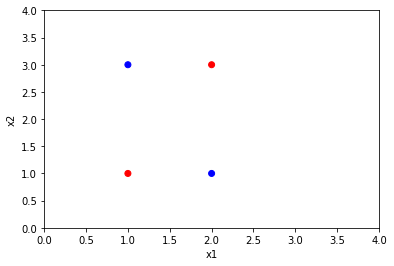
\includegraphics[width=0.4\textwidth]{2Q.png} 
	        \captionsetup{labelformat=empty}
	        \caption{Training set plot}
	        \label{fig: Training set plot}
\end{figure}

	
\end{soln}

\item (Mutual information exercise)  [10 pts] Use the training set Druns.txt.  For the root node, list all candidate cuts and their mutual information.  Hint: to get $\log_2(x)$ when your programming language may be using a different base, use \verb|log(x)/log(2)|.
\begin{soln}
\\For Druns.txt, the root node, candidate cuts (at x1 or x2) and their mutual information is:
\\x1, 0.0, 0.0
\\x1, 0.1, 0.044177
\\x2, -2.0, 0.0
\\x2, -1.0, 0.044177
\\x2, 0.0, 0.0382745
\\x2, 1.0, 0.0048861
\\x2, 2.0, 0.0010821
\\x2, 3.0, 0.0163131
\\x2, 4.0, 0.0494520
\\x2, 5.0, 0.1051955
\\x2, 6.0, 0.1995870
\\x2, 7.0, 0.0382745
\\x2, 8.0, 0.1890526
\end{soln}

\item (The king of interpretability)  [10 pts] Decision tree is not the most accurate classifier in general.  However, it persists.  This is largely due to its rumored interpretability: a data scientist can easily explain a tree to a non-data scientist.  Build a tree from D3leaves.txt.  Then manually convert your tree to a set of logic rules.  Show the tree\footnote{When we say show the tree, we mean either the standard computer science tree view, or some crude plaintext representation of the tree -- as long as you explain the format.  When we say visualize the tree, we mean a plot in the 2D $\x$ space that shows how the tree will classify any points.} and the rules.
\begin{soln}
	 \begin{figure}[h!]
	        \centering
	        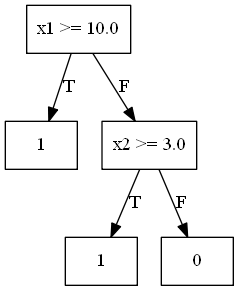
\includegraphics[width=0.4\textwidth]{D3leaves.png} 
	        \captionsetup{labelformat=empty}
	        \caption{Decision tree (D3leaves.txt)}
	        \label{fig:Decision tree (D3leaves.txt)}
	   \end{figure}

	Here, the logic rule is: $ x1 >= 10 \vee x2 >= 3 $ 
\\So, here when $x1 >= 10 $, the value of the first operand in the logic rule becomes 1, and so the tree classfies the input as 1. If not, the tree will check for the values of x2, and based on the value (if $x2 >= 3 $ or not), will give the result.

\end{soln}

\item (Or is it?)  [20 pts] For this question only, make sure you DO NOT VISUALIZE the data sets or plot your tree's decision boundary in the 2D $\x$ space.  If your code does that, turn it off before proceeding.  This is because you want to see your own reaction when trying to interpret a tree.  You will get points no matter what your interpretation is.
And we will ask you to visualize them in the next question anyway.
  \begin{itemize}
  \item Build a decision tree on D1.txt.  Show it to us in any format (e.g. could be a standard binary tree with nodes and arrows, and denote the rule at each leaf node; or Weka style plaintext tree; or as simple as plaintext output where each line represents a node with appropriate line number pointers to child nodes; whatever is convenient for you). Again, do not visualize the data set or the tree in the $\x$ input space.  In real tasks you will not be able to visualize the whole high dimensional input space anyway, so we don't want you to ``cheat'' here.
  \item Look at your tree in the above format (remember, you should not visualize the 2D dataset or your tree's decision boundary) and try to interpret the decision boundary in human understandable English. 
  \item Build a decision tree on D2.txt.  Show it to us.
  \item Try to interpret your D2 decision tree.
  \end{itemize}

\begin{soln}
	\begin{figure}[h!]
	        \centering
	        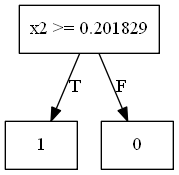
\includegraphics[width=0.2\textwidth]{D1.png} 
	        \captionsetup{labelformat=empty}
	        \caption{Decision tree (D1.txt)}
	        \label{fig:Decision tree (D1.txt)}
	   \end{figure}

	Here, in the D1.txt decision tree, if the value of x2 is $>=$ 0.201829, the input will be classified as 1, if x2 is less than 0.201829, the input will be classified as 0. This dataset is easier to visualise because of the less number of nodes and splits.

          \begin{figure}[h!]
	        \centering
	        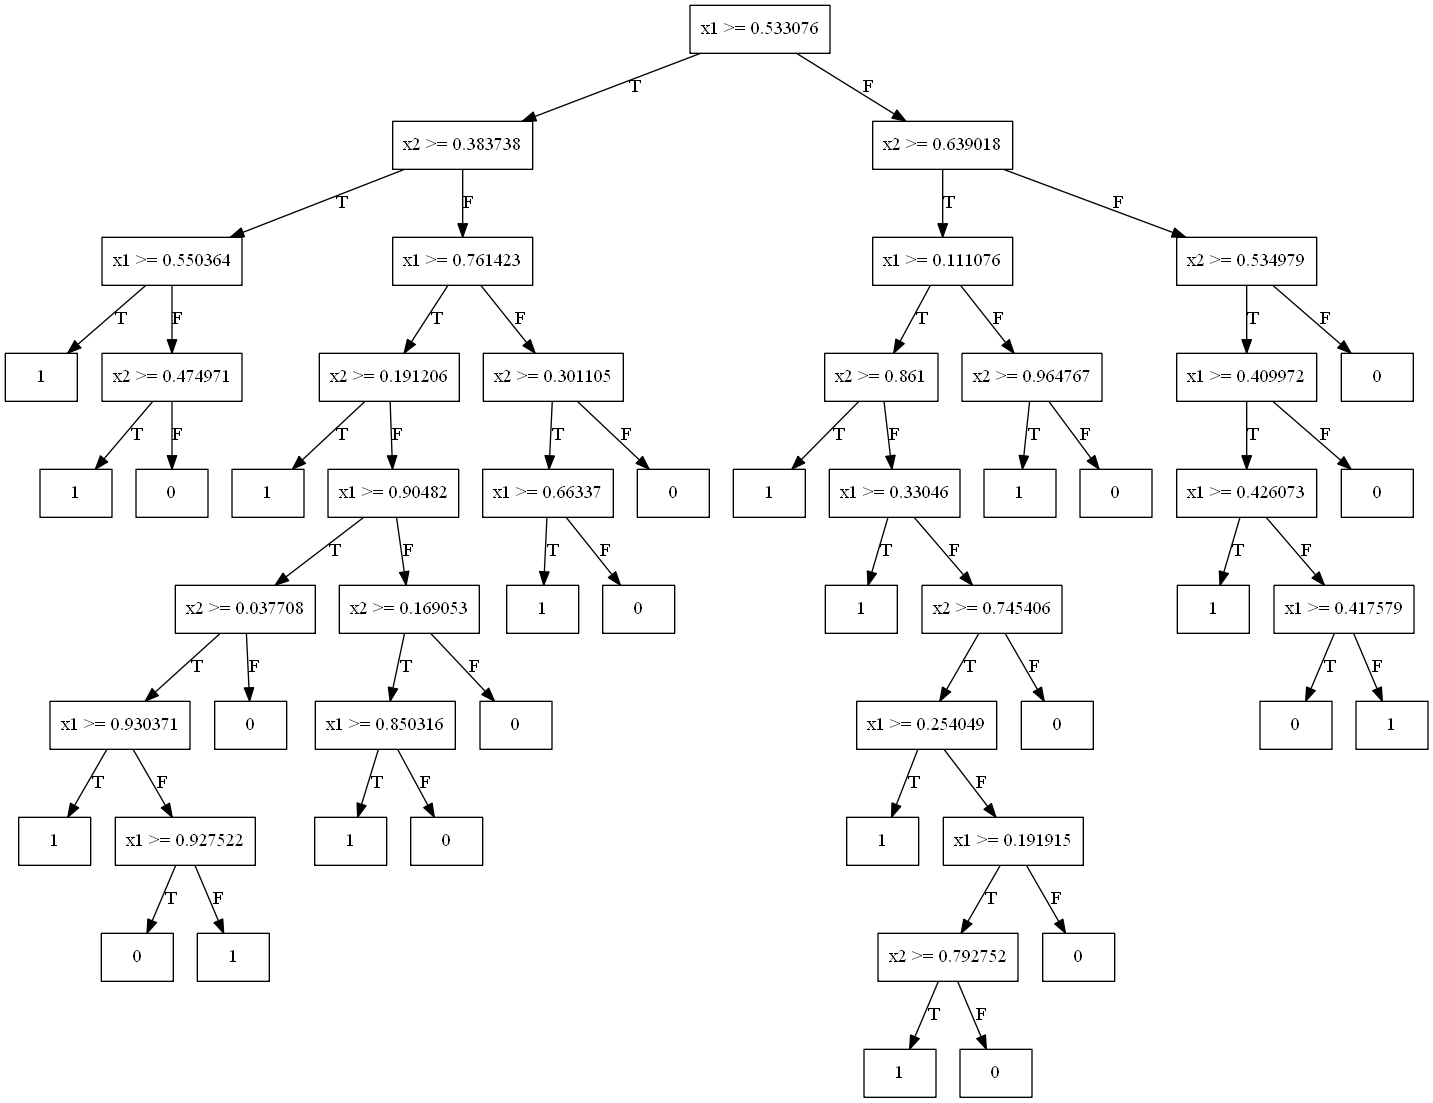
\includegraphics[width=1\textwidth]{D2Tree.png} 
	        \captionsetup{labelformat=empty}
	        \caption{Decision tree (D2.txt)}
	        \label{fig:Decision tree (D2.txt)}
	   \end{figure}
	
Here, in the D2.txt decision tree, the root node splits at x1 $>=$ 0.533076, that is based on x1 $>=$ 0.533076, we move to either the right subtree or the left subtree. The left subtree is further split on the basis of x2 $>=$ 0.383738, while the right subtree is further split on the basis of x2 $>=0.639018$. The subtrees are further split and are ultimately reaching the leaf nodes. Here, there are a lot of nodes in the tree, so its becoming difficult to interpret it by just looking at the decision tree as opposite to a smaller tree with less nodes and splits.   
\end{soln}


\item (Hypothesis space)  [10 pts] For D1.txt and D2.txt, do the following separately:
  \begin{itemize}
  \item Produce a scatter plot of the data set.
  \item Visualize your decision tree's decision boundary (or decision region, or some other ways to clearly visualize how your decision tree will make decisions in the feature space).
  \end{itemize}

Then discuss why the size of your decision trees on D1 and D2 differ.  Relate this to the hypothesis space of our decision tree algorithm. 

\begin{soln}

The size of the decision trees for both D1 and D2 are different. There are a lot of nodes and splits in decision tree of D2.txt, while there is just one in D1.txt decision tree. As seen in the D1 decision boundary, the data is clearly classified on the basis of value of x2. But for D2, the data is not clearly separated based on the values of features x1 and x2. Hence, there are more nodes and splits to accomodate all the different values of the dataset, all the items in the hypothesis space.  

	 \begin{figure}[h!]
	        \centering
	        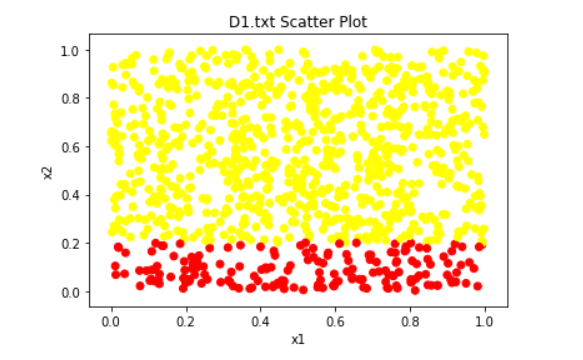
\includegraphics[width=0.4\textwidth]{D1_Scatter.png} 
	        \captionsetup{labelformat=empty}
	        \caption{D1 Scatter Plot}
	        \label{fig:D1 Scatter Plot}
	   \end{figure}
	
	  \begin{figure}[h!]
	        \centering
	        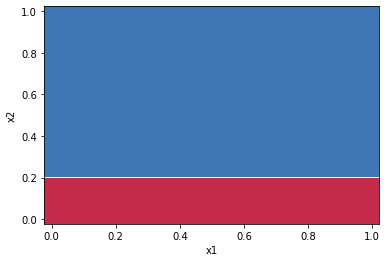
\includegraphics[width=0.4\textwidth]{D1_boundary.png} 
	        \captionsetup{labelformat=empty}
	        \caption{D1 decision boundary}
	        \label{fig:D1 boundary}
	   \end{figure}

	 \begin{figure}[h!]
	        \centering
	        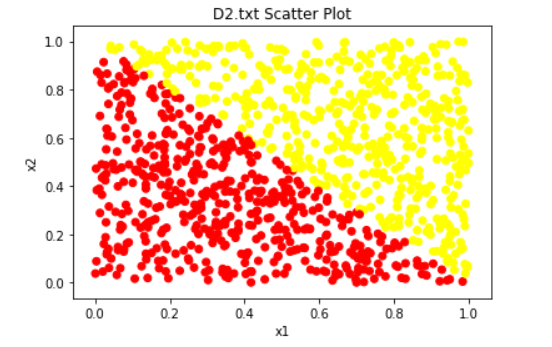
\includegraphics[width=0.4\textwidth]{D2_Scatter.png} 
	        \captionsetup{labelformat=empty}
	        \caption{D2 Scatter Plot}
	        \label{fig:D2 Scatter Plot}
	   \end{figure}	

	
	  \begin{figure}[h!]
	        \centering
	        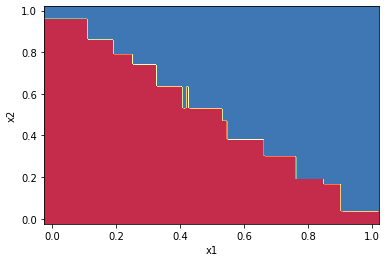
\includegraphics[width=0.4\textwidth]{D2_boundary.png} 
	        \captionsetup{labelformat=empty}
	        \caption{D2 decision boundary}
	        \label{fig:D2 boundary}
	   \end{figure}	

\end{soln}



\item (Learning curve)  [20 pts] We provide a data set Dbig.txt with 10000 labeled items.  Caution: Dbig.txt is sorted.
  \begin{itemize}
  \item You will randomly split Dbig.txt into a candidate training set of 8192 items and a test set (the rest).  Do this by generating a random permutation, and split at 8192.
  \item Generate a sequence of five nested training sets $D_{32} \subset D_{128} \subset D_{512} \subset D_{2048} \subset D_{8192}$ from the candidate training set.  The subscript $n$ in $D_n$ denotes training set size.  The easiest way is to take the first $n$ items from the (same) permutation above.  This sequence simulates the real world situation where you obtain more and more training data.
  \item For each $D_n$ above, train a decision tree.  Measure its test set error $err_n$.  Show three things in your answer: (1) List $n$, number of nodes in that tree, $err_n$. (2) Plot $n$ vs. $err_n$.  This is known as a learning curve (a single plot). (3) Visualize your decision trees' decision boundary (five plots).
  \end{itemize}

\begin{soln}
	

	\begin{table}[htb]
	\centering
	\begin{tabular}{ccc}\hline
	n & test error   \\\hline
	32 & 18.528761061946902  \\
	128 &  10.619469026548673\\
	512 & 8.794247787610619  \\
	2048 & 3.3738938053097347 \\
	8192 & 2.267699115044248\\
	\end{tabular}
	\end{table}

	\begin{figure}[h!]
	        \centering
	        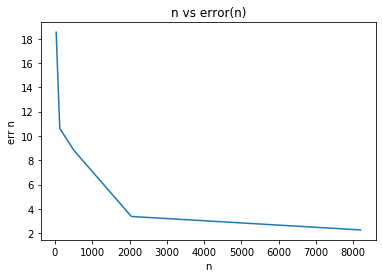
\includegraphics[width=0.6\textwidth]{errorvsn.png} 
	        \captionsetup{labelformat=empty}
	        \caption{Test set error}
	        \label{fig:Test set error}
	  \end{figure}
	
	\begin{figure}[h!]
	        \centering
	        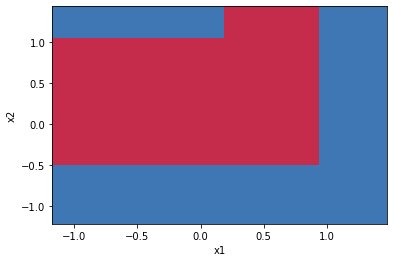
\includegraphics[width=0.4\textwidth]{71.png} 
	        \captionsetup{labelformat=empty}
	        \caption{D32 decision boundary}
	        \label{fig:D32 boundary}
	  \end{figure}	

	\begin{figure}[h!]
	        \centering
	        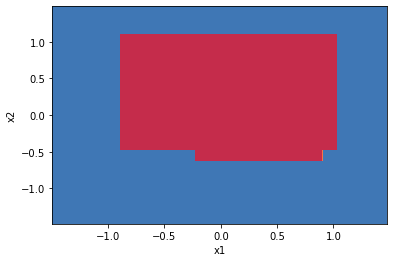
\includegraphics[width=0.4\textwidth]{72.png} 
	        \captionsetup{labelformat=empty}
	        \caption{D128 decision boundary}
	        \label{fig:D128 boundary}
	  \end{figure}

	\begin{figure}[h!]
	        \centering
	        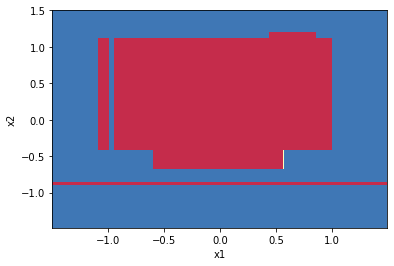
\includegraphics[width=0.4\textwidth]{73.png} 
	        \captionsetup{labelformat=empty}
	        \caption{D512 decision boundary}
	        \label{fig:D512 boundary}
	  \end{figure}

	\begin{figure}[h!]
	        \centering
	        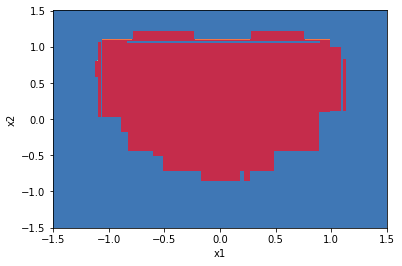
\includegraphics[width=0.4\textwidth]{74.png} 
	        \captionsetup{labelformat=empty}
	        \caption{D2048 decision boundary}
	        \label{fig:D2048 boundary}
	  \end{figure}
	
	\begin{figure}[h!]
	        \centering
	        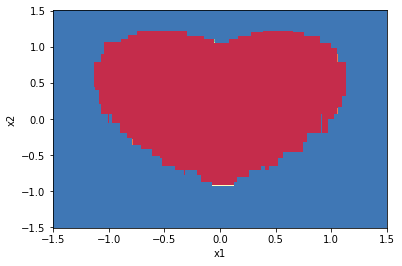
\includegraphics[width=0.4\textwidth]{75.png} 
	        \captionsetup{labelformat=empty}
	        \caption{D8192 decision boundary}
	        \label{fig:D8192 boundary}
	  \end{figure}


\end{soln}


\end{enumerate}

\section{Weka [10 pts]}
Learn to use Weka \url{https://www.cs.waikato.ac.nz/~ml/weka/index.html}.
Convert appropriate data files into ARFF format.
Use trees/J48 as the classifier and default settings.
Produce five Weka trees for $D_{32}, D_{128} \ldots D_{8192}$.  
Show two things in your answer: (1) List $n$, number of nodes in that tree, $err_n$. (2) Plot $n$ vs. $err_n$.

\begin{soln}
\begin{table}[htb]
	\centering
	\begin{tabular}{ccc}\hline
	n & test error (WEKA)   \\\hline
	32 & 19.7456  \\
	128 &  10.1217\\
	512 &  6.4159  \\
	2048 & 2.9867 \\
	8192 & 1.9912\\
	\end{tabular}
	\end{table}

	\begin{figure}[h!]
	        \centering
	        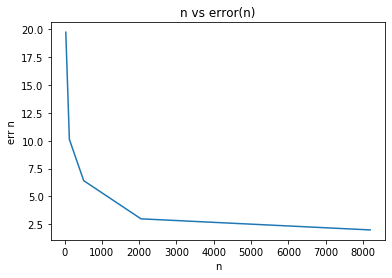
\includegraphics[width=0.6\textwidth]{errorvsnWEKA.png} 
	        \captionsetup{labelformat=empty}
	        \caption{Test set error WEKA}
	        \label{fig:Test set error WEKA}
	  \end{figure}
	

\end{soln}

\bibliographystyle{apalike}
\end{document}
